\documentclass[article,12pt,onesidea,4paper,english,brazil]{abntex2}

\usepackage{lmodern, indentfirst, nomencl, color, graphicx, microtype, lipsum}			
\usepackage[T1]{fontenc}		
\usepackage[utf8]{inputenc}		

\setlrmarginsandblock{2cm}{2cm}{*}
\setulmarginsandblock{2cm}{2cm}{*}
\checkandfixthelayout

\setlength{\parindent}{1.3cm}
\setlength{\parskip}{0.2cm}

\SingleSpacing

\begin{document}
	
	\selectlanguage{brazil}
	
	\frenchspacing 
	
	\begin{center}
		\LARGE SISTEMA DE INFORMAÇÃO GERENCIAL: Análise do sistema utilizado na Secretaria de Planejamento, Orçamento e Gestão – SEPOG/RO1\footnote{Projeto de Pesquisa realizado dentro da Grande Área Organizações Públicas com apoio e supervisão do IFRO Campus Porto Velho Zona Norte.}
		
		\normalsize
	Daiana Cavalcante Gomes\footnote{Colaboradora, daianasabina@gmail.com, Campus Porto Velho Zona Norte.} 
	Jenerson Queiroz Lima Duarte \footnote{Colaborador, jenersonduartee@gmail.com, Campus Porto Velho Zona Norte.} 
	Angelina Maria de Oliveira Licorio\footnote{Orientadora, angelina.licorio@ifro.edu.br, Campus Porto Velho Zona Norte.} 
	Ronilson Oliveira\footnote{Co-orientador, Ronilson.oliveira@ifro.edu.br, Campus Porto Velho Zona Norte.} 
	\end{center}
	
	% resumo em português
	\begin{resumoumacoluna}
		O presente estudo buscou enunciar os indicadores dos sistemas de informação usados pelos servidores Secretaria de Estado de Planejamento, Orçamento e Gestão – SEPOG. Com o advento da renovação tecnológica e concomitante evolução dos meios de comunicação, aumenta a exigência para que os serviços públicos prestados sejam mais ágeis na realização de seus projetos e possibilitem aos gestores o acompanhamento dos processos tornando possível uma melhor tomada de decisão. A pesquisa forneceu indicadores que precisam ser melhorados, aprimorados a fim de fomentar mecanismos que precisam ser ajustados para que o sistema possa atender melhor a demanda em que a SEPOG necessita.
		
		\vspace{\onelineskip}
		
		\noindent
		\textbf{Palavras-chave}: SEPOG. Tecnologia da Informação. Sistema de Informação Gerencial.
	\end{resumoumacoluna}
	
	\textual
	
	\section*{Introdução}
	
	Nos dias atuais a Tecnologia da Informação – TI, é extremamente necessária e indispensável para as instituições públicas tornarem-se cada vez mais integradas entre si. Através da evolução tecnológica e concomitante evolução dos meios de comunicação, as organizações tornaram-se mais ágeis em seus projetos e capazes de envolver seus gestores e trazer informações para o funcionamento de suas operações e tomada de decisão.
	
	O Sistema de Informações Gerencial – SIG fornece dados para o funcionamento da empresa e flui para a melhoria do desempenho das organizações.
	
	No contexto atual a competitividade estimula a busca por melhor desempenho como uma exigência de qualidade.
	
	A SEPOG é um órgão público assistido por uma estrutura tecnológica para o desenvolvimento de suas atividades que são relacionadas ao planejamento, programação, orçamento, acompanhamento e avaliação de programas e projetos. Ela também desenvolve estudos, pesquisas e estatísticas que possibilita a articulação com os municípios e que auxiliam em demais atividades.
	
	\section*{Material e Método}
	
	A Metodologia usada para este estudo inicialmente foi de caráter exploratório, tendo como objetivo levantar as informações necessárias para se familiarizar com a temática em estudo e elaboração do questionário. Os servidores antes de responderem ao questionário são exortados quanto ao termo de consentimento, após o devido preenchimento e assinatura, foi entregue os questionários contendo perguntas abertas e fechadas. Após a conclusão dessa etapa iniciou-se a construção da planilha corresponde ao questionário num software de estatística chamado IBM SPSS 21, responsável pelo tratamento dos dados.
	
	\section*{Resultados e Discussão}
	
	Após a tabulação dos questionários, podemos perceber no gráfico que segue quais são os sistemas de informação usados pelos servidores:
	
	\begin{figure}[!h]
		\centering
		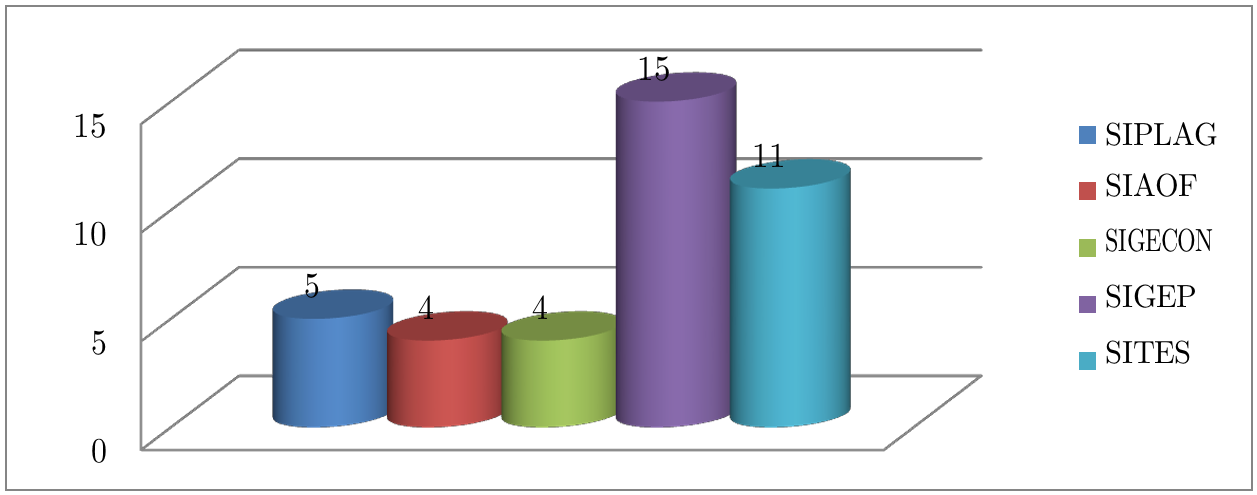
\includegraphics[width=.6\linewidth]{pip-173-1}
		\caption{Sistemas de informação usados pelos servidores.}
	\end{figure}

No próximo gráfico evidencia-se o porcentual de conhecimento que os servidores têm dos sistemas de informações em uso na Secretaria:

\begin{figure}[!h]
	\centering
	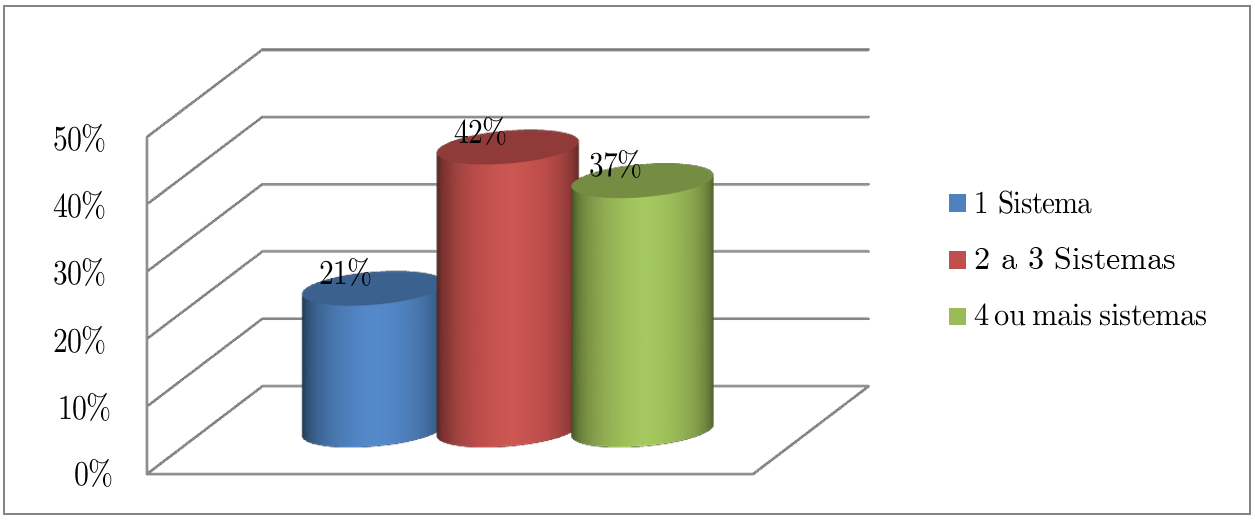
\includegraphics[width=.6\linewidth]{pip-173-2}
	\caption{Sistemas de informação usados pelos servidores.}
\end{figure}

Conseguimos identificar através do próximo gráfico quais são os sistemas de informação mais conhecidos pelos servidores, e em seguida os sistemas de informação mais usados pelos servidores:

	\begin{figure}[!h]
		\centering
		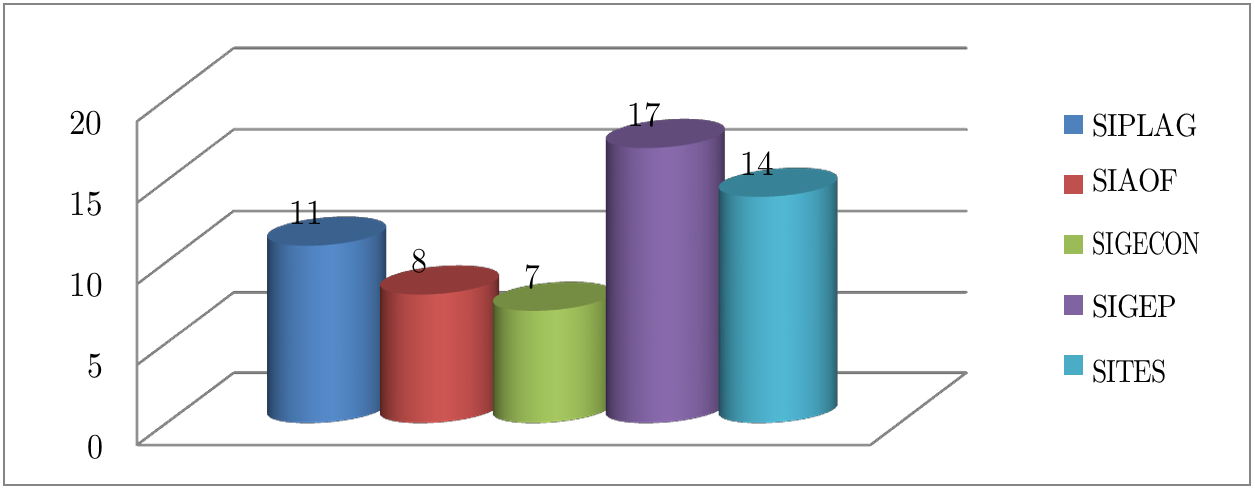
\includegraphics[width=.6\linewidth]{pip-173-3}
		\caption{Sistemas de informação usados pelos servidores.}
	\end{figure}

	\begin{figure}[!h]
	\centering
	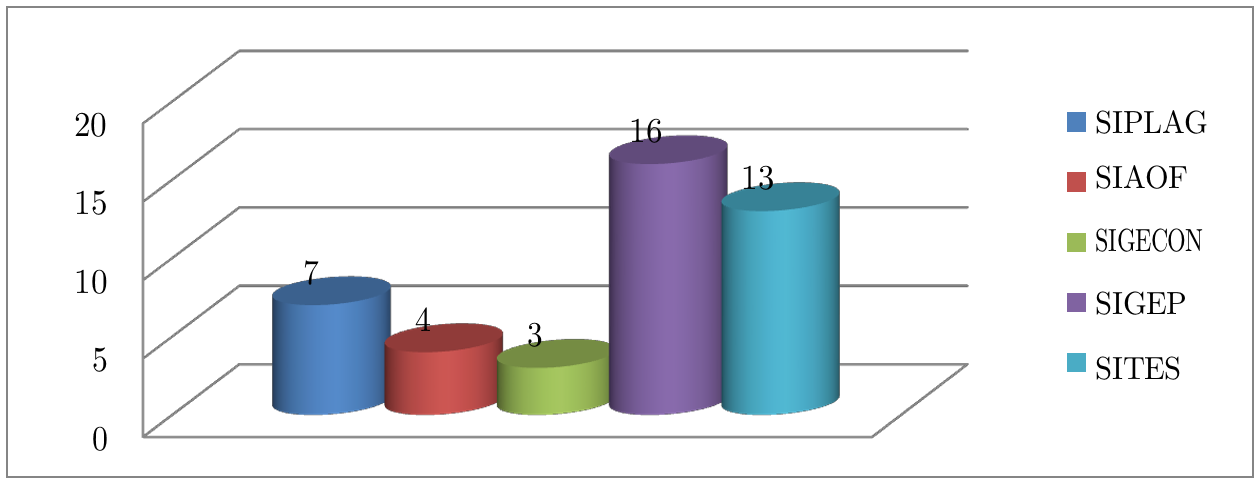
\includegraphics[width=.6\linewidth]{pip-173-4}
	\caption{Sistemas de informação mais conhecido pelos servidores.}
\end{figure}

Alguns servidores relatam dificuldades em algumas singularidades dos sistemas de informação. São elas:

	\begin{figure}[!h]
	\centering
	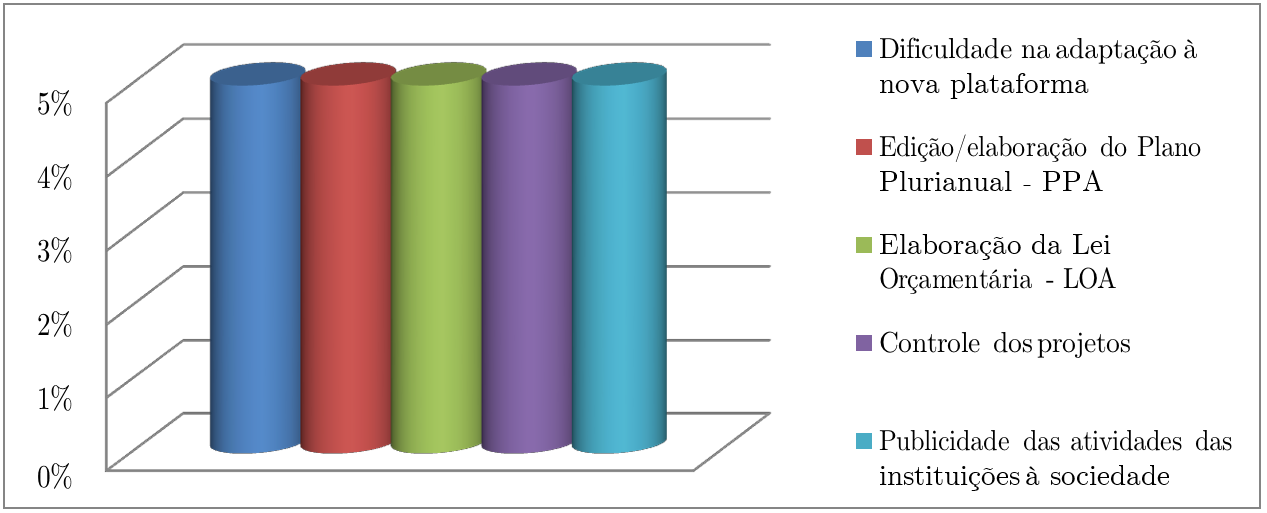
\includegraphics[width=.6\linewidth]{pip-173-5}
	\caption{Dificuldades alegadas pelos servidores.}
\end{figure}


	
	\section*{Conclusões}
	
A pesquisa evidenciou no quadro de servidores da SEPOG a necessidade da troca dos sistemas de informação, e a cada sistema a necessidade de implantação foi diferente. Os servidores que aceitaram fazer parte da pesquisa respondendo ao questionário relataram não haver dificuldade em operar o sistema de informação ao qual trabalha, no entanto quando questionados de forma menos generalizada, uma pequena parte (5\%) respondeu ter duas ou mais dificuldades. É importante salientar que esses servidores alegam ter recebido capacitação no momento da troca de sistemas.
	
	\section*{Instituição de Fomento}
	
O Instituto Federal de Educação, Ciência e Tecnologia de Rondônia, Campus Porto Velho Zona Norte, possibilitou a pesquisa, juntamente com a Secretaria de Estado de Planejamento, Orçamento e Gestão – SEPOG.
	\section*{Referências}
	
	\sloppy
	
	
\noindent ALVES, Christiane Amanda Lima. A importância da tecnologia da informação nas empresas. Disponível em: <http://www.webartigos.com/artigos/a-importancia-da-tecnologia- da-informacao-nas-empresas/95285/>. Acesso em: junho 2016.

\noindent BAZZOTTI, Cristiane \& GARCIA, Elias. Administradores - O Portal da Administração. A Importância do Sistema de Informação Gerencial na Gestão Empresarial para Tomada de Decisões. 2012. Disponível em: < http://www.administradores.com.br/artigos/marketing/a- importancia-do-sistema-de-informacao-gerencial-para-as-empresas/66425/>. Acesso em: maio de 2016.

\noindent OLIVEIRA, Djalma de Pinho Rebouças de. Sistemas de Informações Gerenciais: Estratégicas Táticas Operacionais. 12ª Ed. São Paulo: Editora Atlas, 2008, 299 páginas.

\noindent PAIXÃO, Camila Rangel da Paixão et Al. XXVI ENEGEP. Fortaleza, 2006. Uso estratégico do sistema de informação gerencial: estudo de caso da Petrobrás na unidade de negócios da bacia de Campos (UN-BC). Disponível em:
<http://www.abepro.org.br/biblioteca/enegep2006\_tr530349\_7795.pdf>. Acesso em: junho de 2016.

\noindent REZENDE, Denis Alcides; ABREU, Aline França de. Tecnologia da informação aplicada a sistemas de informação empresariais: o papel estratégico da informação e dos sistemas de informação nas empresas. São Paulo: Atlas, 2000.
\end{document}
